\documentclass{beamer}

\usepackage[utf8]{inputenc}
\usepackage{eurosym}
\usepackage{hyperref}
\hypersetup{
    colorlinks = true
    }
\usepackage{graphicx}

%Information to be included in the title page:
\title{GTA Einführung Robotik mit Makecode}
\author{Mattias Schlenker}
\institute{Wilhelm-Ostwald-Gymnasium}
\date{17. Dezember 2020}

\begin{document}

\frame{\titlepage}

\begin{frame}
\frametitle{Wir programmieren einen Space-Shooter}

Nicht jeder hat einen Roboter abbekommen, zudem haben manche Probleme mit dem UF2-Upload. Also üben wir Makecode, indem wir ein Spiel programmieren. Es soll ein klassischer Weltraumshooter werden: Wir fliegen in Richtung des oberen Bildschirmrandes. Von dort kommen und feindliche Raumschiffe entgegen, mit denen wir nicht kollidieren dürfen, die wir aber abschießen können. 
 
Geht auf \href{https://arcade.makecode.com/}{https://arcade.makecode.com/} und erstellt ein neues Projekt, bspw. ,,GtaAlienShooter''…
 
\end{frame}
 
 \begin{frame}
 \frametitle{Die Szenerie}
 
 Nehmt aus ,,Effekte'' den Effekt für den Startbildschirm und setzt ihn auf den Sternenfeld-Effekt. Aus den ,,Sprites'' holt Ihr  den Block zum erzeugen eines eigenen Sprites. Achtet darauf, dass der Typ auf ,,Player'' steht. Klickt in das graue Feld und malt ein Raumschiff, das auf dem dunklen Hintergrund gut aussieht.
 
 
 \begin{figure}
  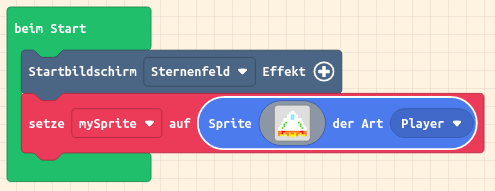
\includegraphics[width=8cm]{game01.png}
  \caption{Startszene}
  \label{fig:game1}
\end{figure}

\end{frame}

 \begin{frame}
 \frametitle{Das Raumschiff bewegen}
 
 Nehmt aus ,,Controller'' den Block für die Bewegung mit Knöpfen, zudem müsst Ihr sicherstellen, dass das Raumschiff innerhalb des Bildschirmes bleibt. Den benötigten Block findet Ihr unter ,,Sprites''.
 
 \begin{figure}
  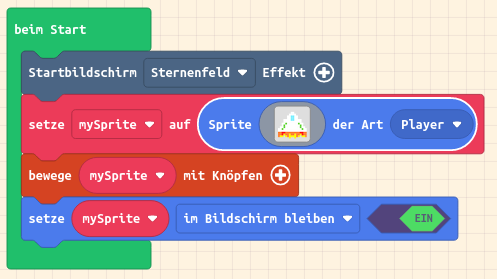
\includegraphics[width=8cm]{game02.png}
  \caption{Mit Steuerung}
  \label{fig:game2}
\end{figure}

\end{frame}

 \begin{frame}
 \frametitle{Alien-Raumschiffe als Gegner}
 Zunächst holen wir einen Block ,,Spielupdate'' und setzen ihn auf eine Sekunde. In diesen kommt ein neues Sprite, das als ,,Projektil von der Seite'' (=Bildschirmrand) definiert ist. Die X-Geschwindigkeit setzen wir auf 0. Im zweiten Block wird die Position des Sprites gesetzt. Für die X-Position ziehen wir dafür aus ,,Mathematik'' eine Zufallszahl, die wir auf 0 bis 160 setzen.
 
 \begin{figure}
  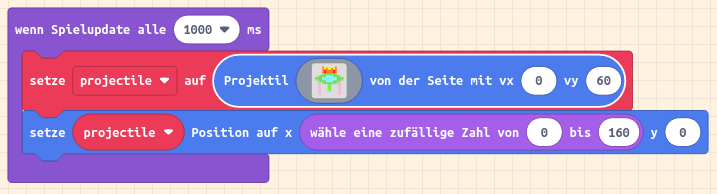
\includegraphics[width=11cm]{game03.png}
  \caption{Alien-Raumschiff}
  \label{fig:game3}
\end{figure}
\end{frame}

 \begin{frame}
 \frametitle{Kollisionserkennung}
 Zuerst müssen wir das gegnerische Raumschiff einer Kategorie zuweisen: ,,Enemy'' (Gegner). Dann holen wir aus ,,Sprites'' den Block für ,,Kollisions-Events'', hier als ,,Überlappung'' definiert und setzen per Dropdown eine Überlappung des eigenen Sprites der Kategorie ,,Player'' mit dem fremden Sprite der Klasse ,,Enemy''.
 
 \begin{figure}
  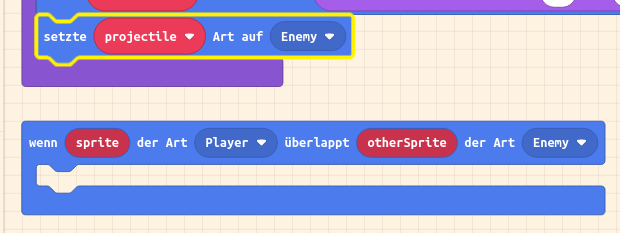
\includegraphics[width=11cm]{game04.png}
  \caption{Kollisionserkennung}
  \label{fig:game4}
\end{figure}
\end{frame}


 \begin{frame}
 \frametitle{Sprite zerstören}
Nehmt nun einen Block ,,Zerstöre'' aus den ,,Sprites'' und zieht dann das ovale ,,otherSprite'' in das ovale Feld im ,,Zerstöre-Block'' - wenn Ihr mögt, bringt ein Klick auf das Plus-Symbol Effekte zum Vorschein:
 
 \begin{figure}
  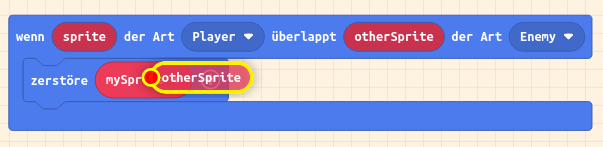
\includegraphics[width=11cm]{game05.png}
  \caption{Kollisionserkennung}
  \label{fig:game4}
\end{figure}
\end{frame}

 \begin{frame}
 \frametitle{Weniger Leben}
Unter ,,Info'' findet Ihr Aktionen und Variablen, die den Spielstand betreffen. Nehmt hier einen Block ,,ändere Leben'' und zieht ihn mit in den Block für das Kollisionsevent. Aus ,,Szene'' könnt ihr passende Effekte auswählen.
 
 \begin{figure}
  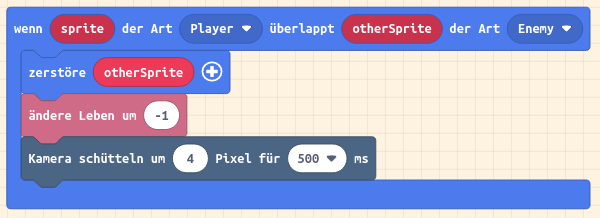
\includegraphics[width=11cm]{game06.png}
  \caption{Weniger Leben}
  \label{fig:game4}
\end{figure}
\end{frame}


 \begin{frame}
 \frametitle{Schießen}
Schießen ist ein ,,Controller-Event'': ,,Wenn A-Taste gedrückt''. Holt aus den ,,Sprites'' nun den Block, der ein Sprite erzeugt, der nicht am Bildschirmrand, sondern in einem anderen Sprite den Ursprung hat, hier in ,,mySprite'', also an der Position des Spielers. Ändert die Leinwandgröße auf 12x12 Pixel und zeichnet etwas Schönes. Ordnet dann das Projektil der Kategorie ,,Projectile'' zu. Optional könnt Ihr den Schüssen Effekte mitgeben. 
 
 \begin{figure}
  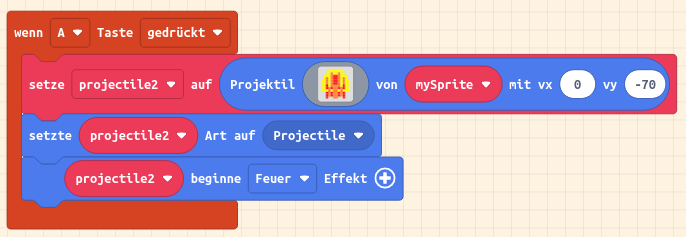
\includegraphics[width=11cm]{game07.png}
  \caption{Schießen mit A}
  \label{fig:game4}
\end{figure}
\end{frame}

 \begin{frame}
 \frametitle{Punkte}
Um mit Spielständen arbeiten zu können, müsst Ihr aus ,,Info'' den Block zur Initialisierung der Punktzahl in den grünen Block ,,beim Start'' ziehen:
 
 \begin{figure}
  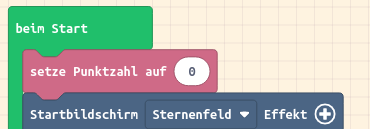
\includegraphics[width=8cm]{game08.png}
  \caption{Punktzahl}
  \label{fig:game4}
\end{figure}
\end{frame}

 \begin{frame}
 \frametitle{Treffer landen}
Für den Treffer benötigt Ihr wieder ein Block für das Überlappungs-Event. Hier sind die Klassen ,,Projectile'' und ,,Enemy'' auszuwählen. Zerstört beide Sprites und erhöht die Punktzahl um 1. 
 
 \begin{figure}
  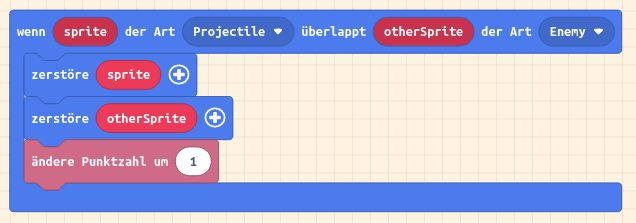
\includegraphics[width=11cm]{game09.png}
  \caption{Punktzahl}
  \label{fig:game4}
\end{figure}
\end{frame}

 \begin{frame}
 \frametitle{Mehr Leben}
Holt diese vier Blöcke aus ,,Mathemathik'', ,,Logik'' und ,,Info'':  
 
 \begin{figure}
  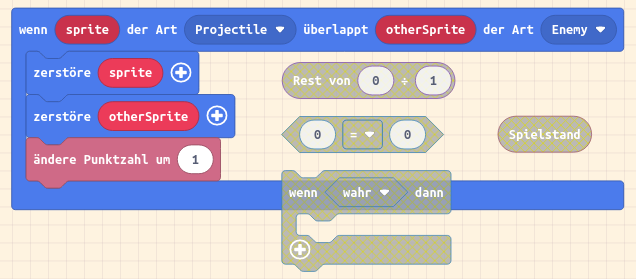
\includegraphics[width=11cm]{game10.png}
  \caption{Vier Blöcke…}
  \label{fig:game4}
\end{figure}
\end{frame}

 \begin{frame}
 \frametitle{Mehr Leben}
Ordnet sie nun so an, dass die Zahl der Leben um 1 erhöht wird, wenn der Rest der Division des Spielstandes durch 20 gleich 0 ist (die Operation ,,Rest nach Division'' heisst auch ,,Modulo''):
 
 \begin{figure}
  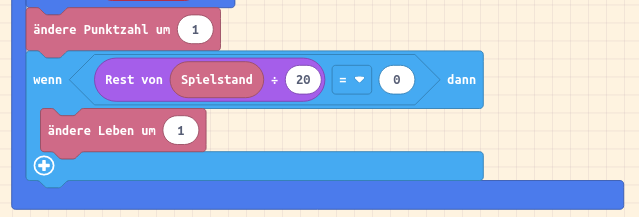
\includegraphics[width=11cm]{game11.png}
  \caption{Mehr Leben}
  \label{fig:game4}
\end{figure}
\end{frame}

\begin{frame}
 \frametitle{Schnellere Gegner}
Um die Geschwindigkeit der Gegner variabel zu machen, benötigen wir eine - richtig Variable. Erzeugt unter ,,Variablen'' eine neue Variable ,,vGegner'' und initialisiert diese im Startblock mit 60.
 
 \begin{figure}
  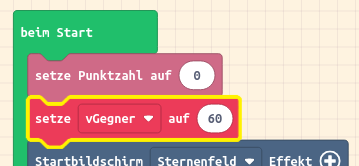
\includegraphics[width=8cm]{game12.png}
  \caption{vGegner}
  \label{fig:game4}
\end{figure}
\end{frame}

\begin{frame}
 \frametitle{Schnellere Gegner}
Im sekündlichen Update wird diese Variable nun ins Feld für ,,vy'' eingesetzt:
 
 \begin{figure}
  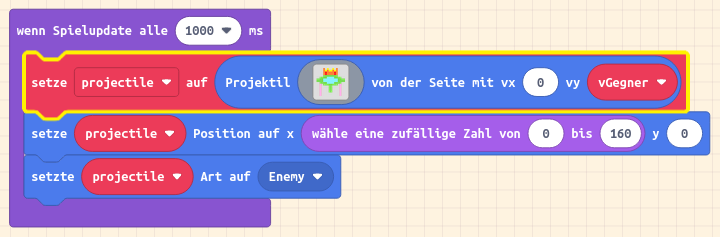
\includegraphics[width=11cm]{game13.png}
  \caption{vGegner}
  \label{fig:game4}
\end{figure}
\end{frame}

\begin{frame}
 \frametitle{Schnellere Gegner}
Und im Block für die Überlappung zwischen ,,Projectile'' und ,,Enemy'' wird mit einer weiteren Modulo-Operation dafür gesorgt, dass Ihr alle 10 Treffer eine neues Leben bekommt. 
 
 \begin{figure}
  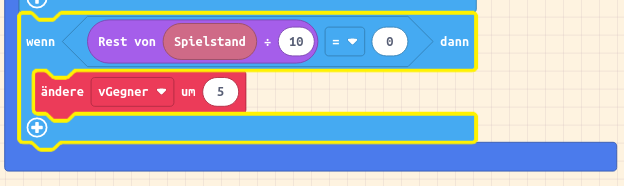
\includegraphics[width=11cm]{game14.png}
  \caption{vGegner}
  \label{fig:game4}
\end{figure}
\end{frame}

\begin{frame}
\frametitle{Fertig!}
Wenn Ihr Euren Code mit meinem vergleichen wollt oder einfach nur spielen möchtet:
   
   \href{https://makecode.com/\_6bUK5eAqF2pu}{https://makecode.com/\_6bUK5eAqF2pu}
\end{frame}

 \begin{frame}
\frametitle{Was habt Ihr gelernt?}
\begin{itemize}
\item Rechteckige Blöcke stehen für Schleifen und Events  
\item Blöcke mit Puzzle-Teil oben und unten gehören in rechteckige Blöcke
\item Blöcke mit spitzer Klammer stehen für Aussagenlogik 
\item Ovale Blöcke rufen Variablen ab oder liefern Ergebnisse von Berechnungen
\item Farbe hilft bei der Zuordnung zu Gruppen
\item Der Modulo-Operator ist praktisch für gegelmäßige Ereignisse  
\end{itemize}
\end{frame}
 
 \begin{frame}
\frametitle{Ideen für Erweiterungen}
Das wurde genannt:

\begin{itemize}
\item Asteroiden, denen man ausweichen muss, die man aber nicht abschießen kann
\item Versorgungsraumschiffe, die die Zahl der Leben erhöhen
\item Spezielle Objekte, die alle Gegner für eine Zeit verlangsamen
\item Mehr Effekte
\item Schöne Start- und Endbildschirme
\item Animation der Sprites, z.b. leichtes Kippen nach rechts oder links bei Bewegung
\item schräg fliegende oder die Richtung ändernde Objekte, denen man ausweichen muss
\item Geschwindigkeitserhöhung nach Zeit und nicht nach Treffern
\item Begrenzte Schusszahl pro Zeiteinheit (ähnlich Token Bucket)
\end{itemize}
\end{frame}
 
  \begin{frame}
\frametitle{Links}
Und hier die Hardware, auf der die Spiele direkt laufen können:

\begin{itemize}
\item \href{https://www.youtube.com/watch?v=uJJlJ_WFcT0}{Meow Bit} 
\item \href{https://www.adafruit.com/product/4242}{PyGamer}
\item \href{https://arcade.makecode.com/hardware/raspberry-pi/wooden-cabinet}{Raspberry Pi}
\end{itemize}

Da bereits der Wunsch geäußert wurde, so ein Arcade-Cabinet zu bauen, ich habe alles vorrätig und wenn sich im Schulclub ein Platz dafür findet, warum nicht einen \href{https://www.thegeekpub.com/4506/build-retropie-bartop-arcade-cabinet/}{eigenen Automaten für die Best-of-WOG-Games?!}

 \end{frame}
\end{document}
